%%%%%%%%%%%%%%%%%%%%%%%%%%%%%%%%%%%%%%%%%%%%%%%%%%%%%%%%%%%%%%%%%%%%%%%%
%                                                                      %
% LaTeX, FIIW thesis template                                          %
% 28/11/2014 v1.2                                                      %
%                                                                      %
%%%%%%%%%%%%%%%%%%%%%%%%%%%%%%%%%%%%%%%%%%%%%%%%%%%%%%%%%%%%%%%%%%%%%%%%
\documentclass[11pt,a4paper]{report}
% Indien je je thesis recto-verso wil afdrukken gebruik je onderstaande opties i.p.v. bovenstaande
%\documentclass[11pt,a4paper,twoside,openright]{report}

\usepackage[a4paper,left=3.5cm, right=2.5cm, top=3.5cm, bottom=3.5cm]{geometry}
\usepackage[dutch]{babel}
\usepackage{graphicx}
\usepackage[latin1]{inputenc}           % om niet ascii karakters rechtstreeks te kunnen inputten
%\usepackage[utf8]{inputenc}            % commentarieer deze regel uit als je utf8 encoded files gebruikt in plaats van latin1
\usepackage{natbib}
\usepackage{listings}



   		% voor het weergeven van broncode
\usepackage{verbatim}					% weergeven van code, commando's, ...
\usepackage{hyperref}					% maak PDF van de thesis navigeerbaar
\usepackage{url}						% URL's invoegen in tekst met behulp van \url{http://}
\usepackage[small,bf,hang]{caption}     % om de captions wat te verbeteren
\usepackage[final]{pdfpages}            % gebruikt voor het invoegen van het artikel in pdf-formaat
%\usepackage{pslatex}					% andere lettertype's dan de standaard types

\usepackage{sectsty}					% aanpassen van de fonts van sections en chapters
\allsectionsfont{\sffamily}
\chapterfont{\sffamily}				%als je hoofsdtuktitels rechts wilt hebben voeg voor \sffamily dit toe: \raggedleft

\usepackage{float}                      % De optie H voor de plaatsing van figuren op de plaats waar je ze invoegt. bvb. \begin{figure}[H]
%\usepackage{longtable}					% tabellen die over meerdere pagina's gespreid worden
%\usepackage[times]{quotchap}           % indien je fancy hoofdstuktitels wil
%\usepackage[none]{hyphenat}
%\usepackage{latexsym}
%\usepackage{amsmath}
%\usepackage{amssymb}

\usepackage{fiiw_gent}
% \usepackage{fiiw_ghent_eng} % For the english version (also change last page at the bottom of this file!

%door onderstaande regels in commentaar te zetten, of op false, kan je pagina's weglaten
%bijvoorbeeld het weglaten van een voorwoord, lijst met symbolen, ...
%%%%%%%%%%%%%%%%%%%%%%%%%%%%%%%%%%%%%%%%%%%%%%%%%%%%%%%%%%%%%%%%%%%%%%%%%%%%%%%%%%%%%%%%
%voorwoord toevoegen?
\acknowledgementspagetrue
\acknowledgements{voorwoord}			%.tex file met daarin het voorwoord
%abstract toevoegen?
%\abstractpagetrue
%\abstracts{abstract}					%.tex file met daarin het abstract
%lijst van figuren toevoegen?
\listoffigurespagetrue
%lijst van tabellen toevoegen?
\listoftablespagetrue
%lijst van symbolen toevoegen?
%\listofsymbolspagetrue
%\listofsymbols{symbolen}				%.tex file met daarin de lijst van symbolen



%informatie over het eindwerk, de promotor, ...
%%%%%%%%%%%%%%%%%%%%%%%%%%%%%%%%%%%%%%%%%%%%%%%
\opleiding{}
\afdeling{Elektronica-ICT}

\title{Robot Bartje\\The Robot Champion of 3ElictE}
\subtitle{ }
% \author{naam student}
\forenameA{Tom}
\surnameA{Lierman}
\forenameB{Matthias}
\surnameB{Alleman}
\academicyear{2017 - 2018}

\promotorA[Begeleiders]{Guus Leenders\\ Stijn Crul \\ Carine Naessens\\ Liesbet Van der Perre}
\promotorB[Coach]{Kevin Verniers\\ }

\begin{document}
\selectlanguage{dutch}
% \selectlanguage{english} % For the english version
\preface
%second chapter of your thesis
\chapter{Dankwoord}
Graag willen wij enkele mensen bedanken die ons de afgelopen maanden geholpen hebben met ons project.
Om te beginnen willen we Guus Leenders en Stijn Crul bedanken daar ze ons geholpen hebben met het 3D-printen van onderdelen. Dit waren ook de hoofdbegeleiders van het project bij wie we terecht konden met vragen over de opdracht . We willen verder ook onze coach Kevin Verniers bedanken bij wie we altijd terecht konden met vragen over de uitwerking van de robot. We bedanken als laatste onze klasgroep, iedereen hielp elkaar met kleine vraagjes en problemen.


%Het eerste hoofdstuk van je thesis.
\chapter{Opdrachtbeschrijving}
\label{chap:Opdrachtbeschrijving}
De opdracht bestaat eruit om een line-following robot te maken. Deze robot wijkt enigszins af van de klassieke line-follower aangezien de parcours die wij moesten kunnen afleggen, bestonden uit 2 volle buitenlijnen en een gestreepte middellijn, waardoor we niet zo maar de middellijn konden volgen. De onderbrekingen maakten een algoritme tot het volgen ervan zeer ingewikkeld en onvoorspelbaar. We kregen op voorhand 3 verschillende circuits die de robot autonoom zou moeten afleggen terwijl hij simultaan andere taken uitvoert zoals snelheden registreren en doorsturen of RFID-tags uitlezen en doorsturen. De breedte van de baan is ongeveer twee keer de breedte van de auto. We kregen een basispakket vanwaar we konden vertrekken dewelke bestond uit het chassis van de robot, 2 motoren, een batterij, een ArduMoto shield en 2 Arduino Uno's. We kregen ook een 3D-printer ter beschikking om 3D-onderdelen de printen die we nodig hadden om sensoren te bevestigen en dergelijke. Verder kregen we ook nog een budget van 50 euro van de school om ons te voorzien van de nodige componenten. De opdracht bestaat zowel uit het bedenken en ontwerpen van de nodige hardware als het schrijven van de nodige software zodat de robot de 3 verschillende circuits autonoom kan afleggen.
\section{Hardware}
Voor het ontwikkelen van de Software konden we beroep doen op een Arduino Uno van..... en een Motorshield van Sparkfun, zoals te zien in Figuur ~\ref{fig:ArduMoto}, maar voor de uiteindelijke opdracht moesten we natuurlijk gebruik maken van printplaten de we zelf vervaardigd hadden. Aan de hand van een schema van de Arduino Uno, dat we konden downloaden van het internet, konden we onze eigen PCB ontwerpen waarbij we alle niet-noodzakelijke componenten weglieten en de L298 Chip toevoegden voor de aansturing van de motoren. Voor de sensoren, Bluetooth-module en RFID-reader waren we vrij om te kiezen welke we kochten of deze zelf maakten.




\begin{figure}[H]
\centering
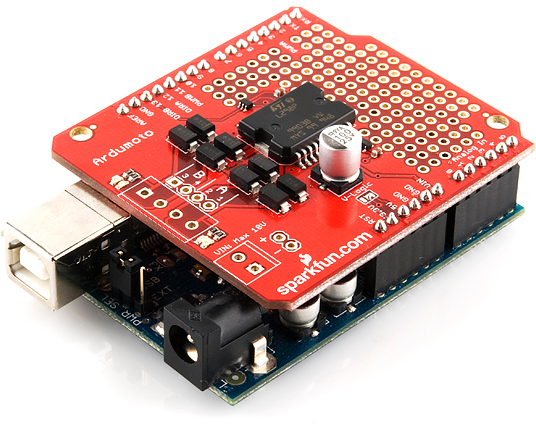
\includegraphics[width=0.75\textwidth]{ArduMoto.png}
\caption{Motorshield gecombineerd met een Arduino. \label{fig:ArduMoto}}
\end{figure}

\section{Software}
Het tweede onderdeel van de opdracht bestond erin om de Arduino (en dus later ook onze eigen PCB) dusdanig te programmeren dat hij autonoom verschillende circuits kon afleggen in een zo kort mogelijke tijd. Er werd ons aangeraden te werken met een PID-regeling om een zo stabiel mogelijke robot te verkrijgen. Tijdens het afleggen van het circuit, moest de robot in staat zijn om zijn snelheid te meten, RFID-tags uit te lezen en van beide, de data , via Bluetooth, door te sturen naar een Raspberry Pi.
%In dit hoofdstuk\index{hoofdstuk} gaan we een voorbeeld geven van een voetnoot\footnote{Dit is dus een voetnoot}. Een referentie naar hoofdstuk ~\ref{verwijzing}, dat zich op pagina \pageref{verwijzing} bevindt, is dus ook een koud kunstje. Zorg er wel voor dat je de namen van de labels een beetje verstandig kiest. Hoofdstukken label je het best als hfdstk:naam, plaatjes als img:naam en tabellen\index{tabellen} als tabel:naam. Zo verlies je zelf de bomen in het bos niet.
%\newpage
%SDffjfhd fsffh hsf
%fh fhf
%shf klfh
%ffffsdfklfhklfhklfhhfklfhkldhffhsdfhfhfhfhfh
%\newpage
%dhfhffh hf fh fh fhfh fhfh hfh fhffhsdfhfhfhfhfhfhsdfh hfh fh
 




%second chapter of your thesis
\chapter{Planning}
We hebben een korte planning opgesteld en weergegeven in figuur~\ref{fig:planning}. We hebben eerst ruim de tijd genomen om het probleem uitgebreid te analyseren en de beste manier te bepalen om te werk te gaan. We konden vrij snel het eerste circuit afleggen maar we hebben dan ook nog proberen de PID-regeling te perfectioneren vooraleer we naar volgende circuits over gingen. Dit is dus ook de reden dat we redelijk lang bezig hebben gebleven op het eerste, simpelste circuit. We hebben deze planning algemeen gezien zeer goed kunnen volgen.
\begin{figure}[h]
\centering
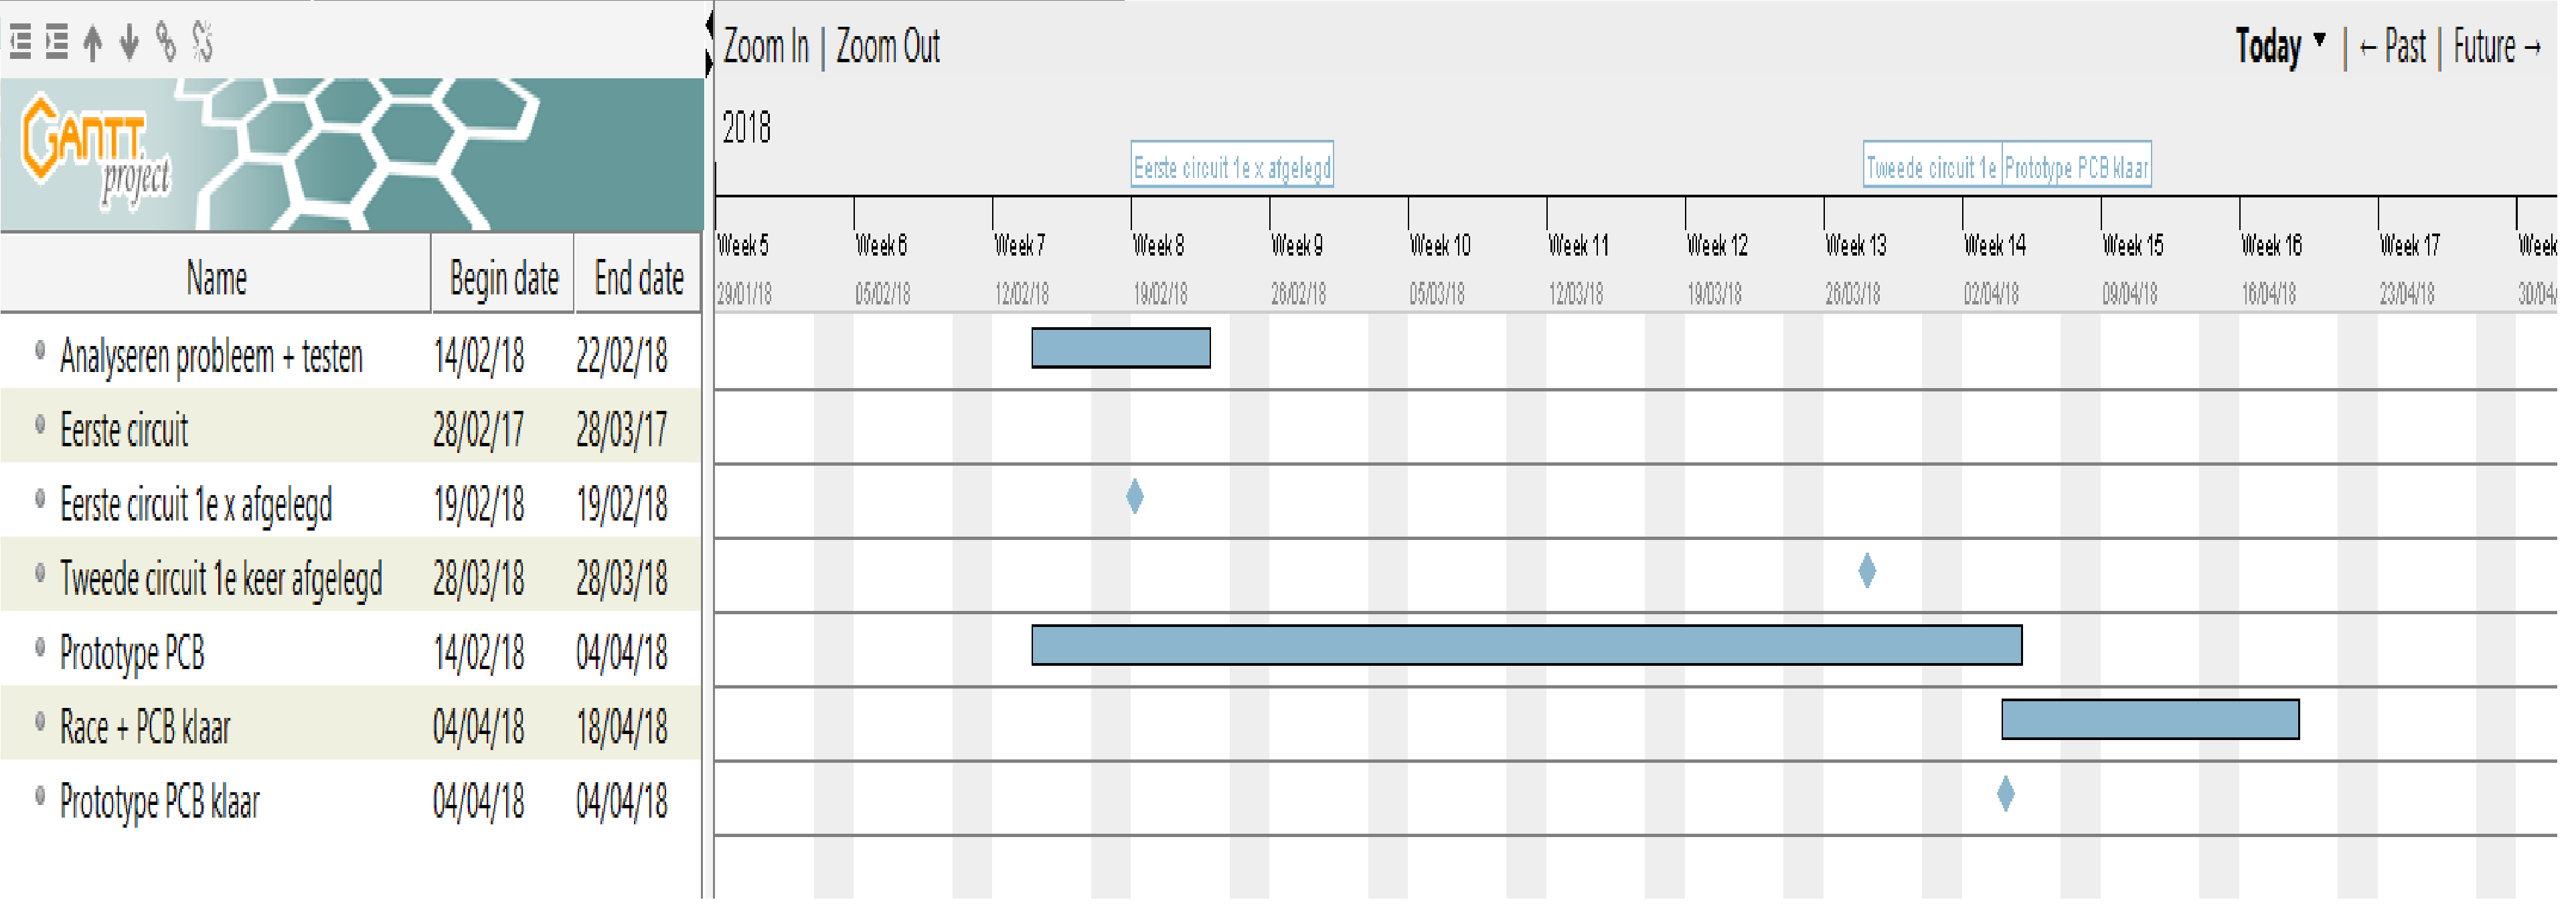
\includegraphics[width=1\textwidth]{planning.png}
\caption{Planning met milestones}
\label{fig:planning}
\end{figure}

%second chapter of your thesis
\chapter{Onkosten}
In het vorig hoofdstuk hebben we naar deze tekst verwezen\label{verwijzing}.

%%%%%%%%%%%%%%%%%%%%%%%%%%%%%%%%%%%%%%%%%%%%%%%%%%%%%%%%%%%%%%%%%%% 
%                                                                 %
%                            CHAPTER                              %
%                                                                 %
%%%%%%%%%%%%%%%%%%%%%%%%%%%%%%%%%%%%%%%%%%%%%%%%%%%%%%%%%%%%%%%%%%% 
 
\chapter{Vormgeving van de Robot}
 
%You can say great work has been done about something \citep{Castleman98,Granlund95} or say that \citet{Holmes95} did something really great.




Alvorens aan te vangen met het schrijven van de software en het ontwerpen van de PCB hebben we onderzocht hoe de ideale robot er zou moeten uitzien om het parcours foutloos en zo snel mogelijk te kunnen afleggen. Een eerste keuze die we moesten maken was of we het losse wieltje vooraan of achteraan wilden plaatsen. We bekeken beide situaties en besloten dat het losse wieltje vooraan de beste oplossing was aangezien de sensoren zich dan op een grotere afstand bevinden van de stuurwielen. De afstand van sensor tot de stuurwielen zorgt ervoor dat de kleinste fout reeds tot uiting komt en de wielen dus sneller correcties kunnen uitvoeren zodat de fout minimaal blijft. Ook bij de keuze van de geschikte arm zal blijken dat we de afstand tussen de stuurwielen en de sensoren trachten te maximaliseren.


We hadden als oorspronkelijk doel om onze robot autonoom de circuits te laten rijden met behulp van 1 arm van 13 cm waarop 3 sensoren bevestigd zijn zoals te zien in Figuur~\ref{fig:3sensoren}. We hebben dan ook zo snel mogelijk deze arm ontworpen en geprint met de 3D-printer zodat wij onmiddellijk konden beginnen met het ontwerpen van de software en het afstellen van de motoren en de sensoren met behulp van PID waarden. Nadat we deze arm aan de rechterkant hadden bevestigd, ging het allemaal vrij snel en hadden we in een mum van tijd een robot die het eerste circuit, het ovale, vloeiend kon afleggen zonder van het parcours te komen. De arm stond 90$^\circ$ gedraaid ten opzichte van de langsas van onze Robot waardoor we de afstand tussen de stuurwielen en de sensoren niet konden maximaliseren. Nadat we de arm onder een hoek van ongeveer 30$^\circ$ ten opzichte van de langsas van de robot geplaatst hadden, merkten we een grote prestatieverbetering op en konden we de snelheid opdrijven.



\begin{figure}[H]
\centering
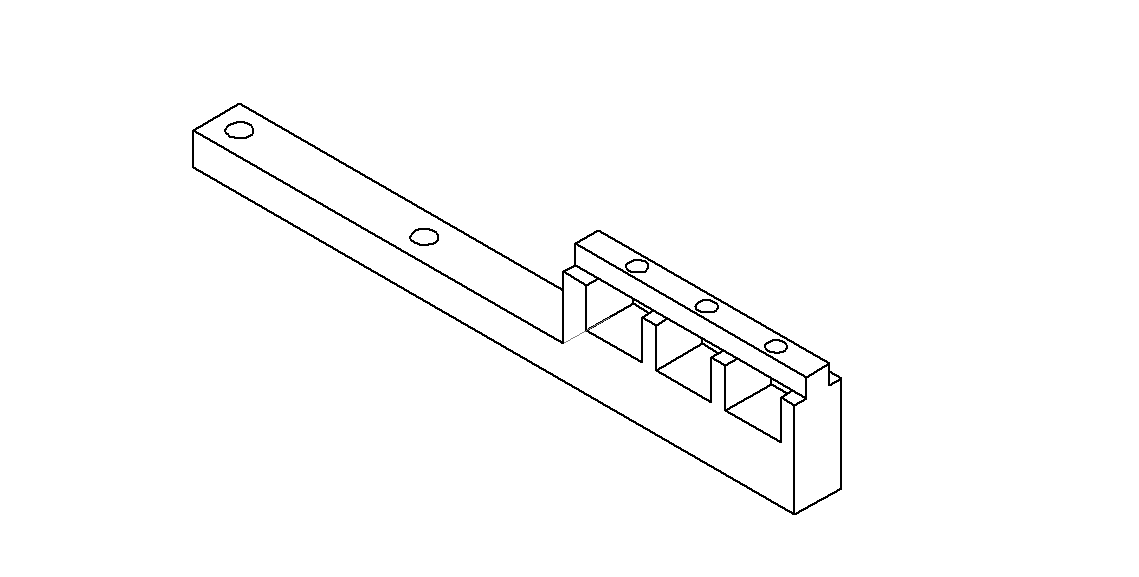
\includegraphics[width=0.75\textwidth]{3sensoren.png}
\caption{Arm voor 3 sensoren. \label{fig:3sensoren}}
\end{figure}


Ons ontwerp was momenteel enkel nog maar in staat om bochten te nemen in 1 richting, namelijk tegenwijzerzin, wanneer we de buitenbochten volgden. We begrepen dat ons ontwerp nog niet voldeed om de ingewikkeldere circuits af te leggen waarbij er zowel bochten naar links als naar rechts zouden voorkomen. We hebben vervolgens onderzoek gedaan om de optimale arm te ontwerpen.

De tweede arm die we ontwikkelden kon plaats bieden aan 5 sensoren en moest onder eenzelfde hoek geplaatst worden als de bovenstaande arm. We ondervonden echter dat de 2 extra sensoren geen meerwaarde konden bieden aangezien we geen extra foutsituaties konden defini\"eren in onze software omdat de arm niet buiten het circuit mocht komen. 

Ons laatste ontwerp bestond uit 2 armen, die elkaars spiegelbeeld zijn en waarbij de top van de arm opnieuw een hoek van 30$^\circ$ maakt met de langsas van de robot. U kan dergelijke arm vinden in Figuur \ref{fig:schuinnaarvoor}. Ons doel was dat de armen van de robot zich zo dicht mogelijk bij de buitenlijnen van het circuit bevonden zodat, wanneer de robot afwijkt van de lijn, dit niet zou resulteren in een te grote afwijking van zijn richting. Daarom bezit de arm eerst nog een stuk van 5 cm in de dwarsrichting van de robot zodat de ene arm zich maximaal 2 cm van de buitenlijn bevindt, wanneer de andere zich op de lijn bevindt. Deze armen bleken voor ons project optimaal en gebruikten we dan ook in ons eindontwerp.

\begin{figure}[H]
\centering
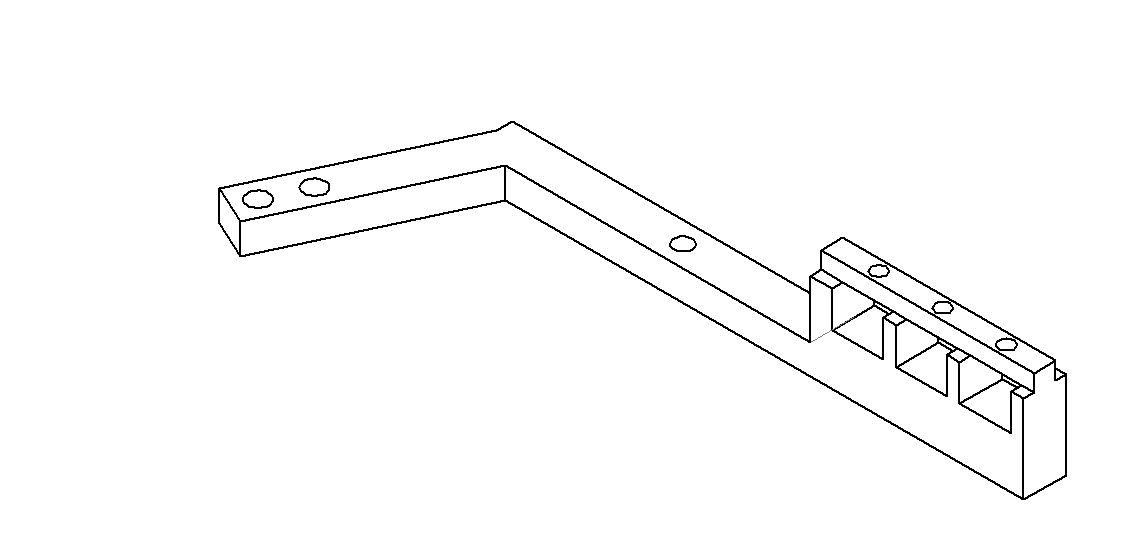
\includegraphics[width=0.75\textwidth]{schuinnaarvoor.png}
\caption{Arm voor sensoren die we gebruiken in ons eindontwerp \label{fig:schuinnaarvoor}}
\end{figure}

We ontwierpen verder ook nog een houdertje voor de RFID-reader zodat deze zich net voor het losse wieltje zou bevinden. Dit is de plaats waar de robot, en dus ook de RFID-tag, zich met grootste zekerheid boven de lijn bevindt.

Om de snelheid van onze robot te meten, maakten we gebruik van eenzelfde infrarood sensor als de sensoren voor het registreren van de witte lijn. We printten een zwart schijfje met de 3D-printer en maakten een spie van de schijf wit zodat de sensor het wit kon waarnemen en op die manier telkens een rotatie van het wiel kon registreren. De sensor zelf hebben we subtiel met een klein houdertje bevestigd onder de robot.

Als laatste gaven we de robot nog vorm met 2 verlengstukjes om een extra printplaat, bedoeld om de bedrading overzichterlijker te maken, te bevestigen en een houder voor de batterij, zodat we deze onderaan konden bevestigen en deze niet meer in de weg zou liggen.

Voor de vormgeving hebben we dus rijkelijk gebruik gemaakt van de 3D-printer waardoor we alles konden positioneren op de exacte plaats waar we het wilden waardoor de robot een afgewerkt geheel werd.



 
%\begin{figure}
%\vspace{2.0in}
%\caption{This is the Caption for Figure 1}
%\end{figure}

 
%\begin{table}[top]
%\begin{center}
%\begin{tabular}{lll}
%Here's       & an          & example  \\
%of           & a           & table    \\
%floated      & with        & the      \\
%\verb+table+ & environment & command.
%\end{tabular}
%\end{center}
%\caption{This is the Caption for Table 1}
%\end{table}
 
%xxx xxxxx xxxxx xxx xxxx xxxx xxxxx xxxxx xxxx xxxxx xxxx xxxxxxxxx
%xxx xxxxx xxxxx xxx xxxx xxxx xxxxx xxxxx xxxx xxxxx xxxx xxxxxxxxx
 	 
%second chapter of your thesis
\chapter{Hardware}
Voor onze robot maken we gebruik van 3 zelfgemaakte PCB$\prime$s. Twee ervan zijn de combinatie van de Motorshield en de Arduino/Atmega en de andere is een printplaat om de bekabeling te reduceren.





\section{Tussenstuk}
We maken gebruik van een tussenstukje, zodat alle line-following sensors naar hetzelfde printplaatje gaan en dit printplaatje dan enkel met 1 voeding en 1 ground moet verbonden worden. De uitgangssignalen worden hier gewoon doorgegeven naar de Atmega. We hebben op dit printplaatje ook de mogelijkheid voorzien om de Bluetooth-module en de RFID-reader aan te sluiten. We hebben nadien ontdekt dat de RFID-reader niet echt kon aangesloten worden op dit printplaatje, om de simpele reden dat het gebruik maakt van dezelfde pinnen die we nodig hebben voor de motoraansturing. Dit leggen we later nog uitgebreider uit. 






We hebben dus 10 5V-aansluitingen voorzien, 10 GND-aansluitingen, de outputs van de sensors die doorgestuurd kunnen worden, de pinnen nodig voor de Bluetooth-module (Key, Vcc, GND, TXD, RXD en State) en de signalen nodig voor de RFID-reader, maar dit wordt niet gebruikt. Niet alle zes de uitgangen van de Bluetooth-module moeten worden doorgestuurd naar onze atmega, deze vereenvoudiging vindt ook plaats op deze PCB. Enkel de signalen Vcc, GND, TXD en RXD worden van een uitgang voorzien. Deze uitgangen worden dus doorverbonden met de Atmega. De Vcc en de GND aan deze uitgang zorgen dus ook voor de voeding van de volledige PCB. We maken gebruik van de HC05 Bluetooth-module, een foto van de module wordt weergegeven in afbeelding~\ref{fig:HC05}.
\newpage
\begin{figure}[h]
\centering
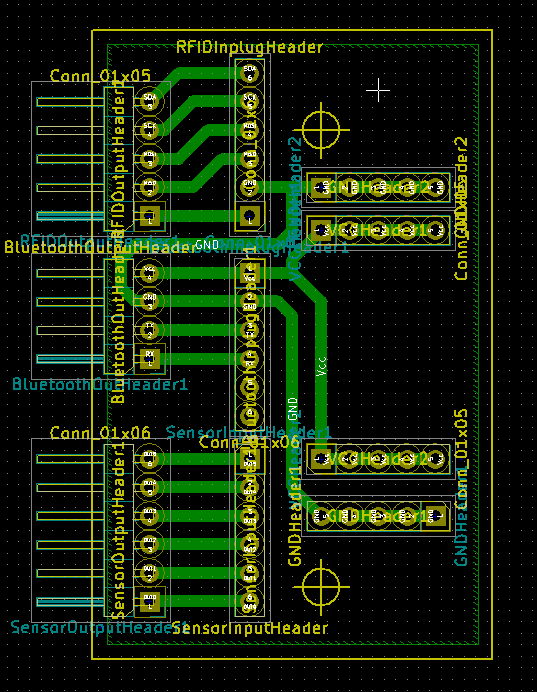
\includegraphics[width=0.3\textwidth]{tussenstukPCB.png}
\caption{Routing van de PCB die als verlengstuk dient. \label{tussenstukPCB}}
\end{figure}


\begin{figure}[h]
\centering
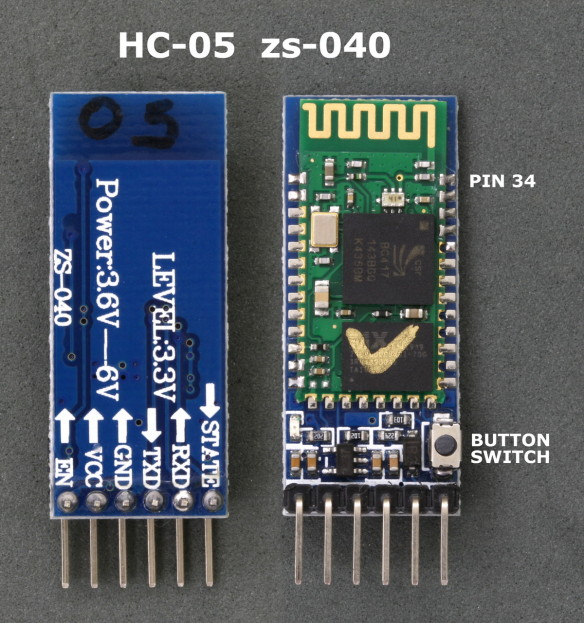
\includegraphics[width=0.3\textwidth]{HC05.jpg}
\caption{De gebruikte Bluetooth-module, ingeplugd op de verlengPCB.}
\label{fig:HC05}
\end{figure}
\section{Ardumoto}
\subsection{Ardumoto RFID}
De tweede printplaat die we gebruiken is eigenlijk ook de volledige combinatie van de atmega en de motorshield, maar we gebruiken enkel de atmega. Deze PCB zorgt voor de aansturing van de RFID-reader. We hebben een tweede atmega nodig omdat de RFID-reader volgende signalen nodig heeft om correct aangestuurd te worden: SS/RX, SCK, MOSI, MISO/TX, IRQ, GND, RST, Vcc. 3 van deze pinnen worden ook gebruikt voor de motoraansturing. SCK is namelijk dezelfde pin als die voor de aansturing van de richting van motor B. MOSI is dezelfde pin als die voor de aansturing van de snelheid van motor B. En de laatste overeenkomstige pin is die van MISO, dit is namelijk dezelfde pin als de aansturing van de richting van motor A. Over deze signalen kunnen er geen twee signalen tergelijkertijd worden over gestuurd. We konden ook eventueel gebruik maken van het $I^{2}C$ principe, in plaats van ISP. Door $I^{2}C$ te gebruiken gingen we geen pinnen nodig hebben die we al gebruikt hadden en dus ook geen tweede PCB, maar we waren toen al beter aan een wat verbeterde versie van de PCB waardoor we dus toch twee werkende PCB$\prime$s gingen hebben. We hadden ook al een werkende code voor de RFID gebasseerd op het ISP protocol. We hebben gebruik gemaakt van een RFID-reader-module, nl. de MRFC522, deze module wordt weergegeven in figuur~\ref{fig:MRFC522}. Om een RFID uit te lezen moet de reader op $\approx$ 1 cm passeren boven de tag. Dit probleem hebben we opgelost door een stukje te laten printen die we vastvijzen aan het wagentje.
\begin{figure}[h]
\centering
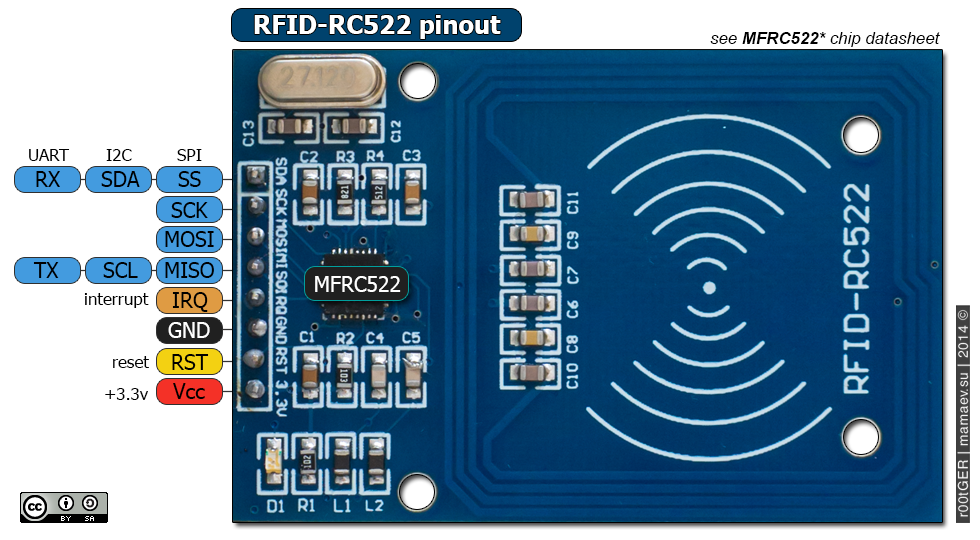
\includegraphics[width=0.75\textwidth]{MRFC522.png}
\caption{Gebruikte RFID-reader MRFC522. \label{fig:MRFC522}}
\label{fig:ACEquiv}
\end{figure}
\subsection{Ardumoto Motor}
Deze PCB dient voor de aansturing van de motoren en ook het doorsturen van de signalen naar de Raspberry Pi via de Bluetooth module. Er waren nog enkele fouten gekropen in het PCB-design. Enkele footprints waren aan de kleine kant, terwijl we dachten na de eerste keer we ze wat aangepast hadden. Maar de grootste fout die erin zat was dat we een ingang van de L298 (de IC verantwoordelijk voor de motoraansturing) vergeten te verbinden waren met het PWRIN signaal. \\
Als basis van ons schema hebben we gebruik gemaakt van een Arduino Uno. Om te beginnen konden we de USB interface voor de aansluiting van een USB-kabel weglaten. (FOTO USB) Dit konden we weglaten doordat we gebruik gingen maken van de ICSP-pinnen mbv. een andere Arduino. We hebben ook bewust alle LED$\prime$s weggelaten omdat we dit niet echt nodig hebben en dit onze arduino groter zou maken dan strikt nodig. We hebben ook de labels verandert van het standaardschema naar wat meer betekenisvolle namen zoals bijvoorbeeld MISO vervangen door DIR A. (FOTO ATMEGA) R8 bijvoorbeeld hebben we ook weggelaten, deze weerstand wordt vaak gebruikt om een brugje te cre$\ddot{e}$ren om baantjes te kunnen ondertrekken. Pinnen 27 en 28 hebben we niet nodig, dus mogen we de condensator hier rond ook verwijderen. De jumper hebben we weggelaten omdat we die niet nodig achtten. 

%In het vorig hoofdstuk hebben we naar deze tekst verwezen\label{verwijzing}.

%second chapter of your thesis

\chapter{Software}

\section{Arduino}

In onze code hebben we er voor geopteerd om zo veel mogelijk gebruik te maken van zelfgemaakte bibliotheken om zo de onderdelen van ons programma zo goed mogelijk van elkaar te scheiden zodat er zo weinig mogelijk verwarring mogelijk is bij het bestuderen van de code. We gebruiken dan ook slechts 1 lijn code in ons .ino bestand om een bibliotheek aan te roepen van waaruit vervolgens het hele programma wordt aangestuurd. In Figuur \ref{fig:flowchart} vindt u de flowchart van ons programma.

\begin{figure}[h]
\centering
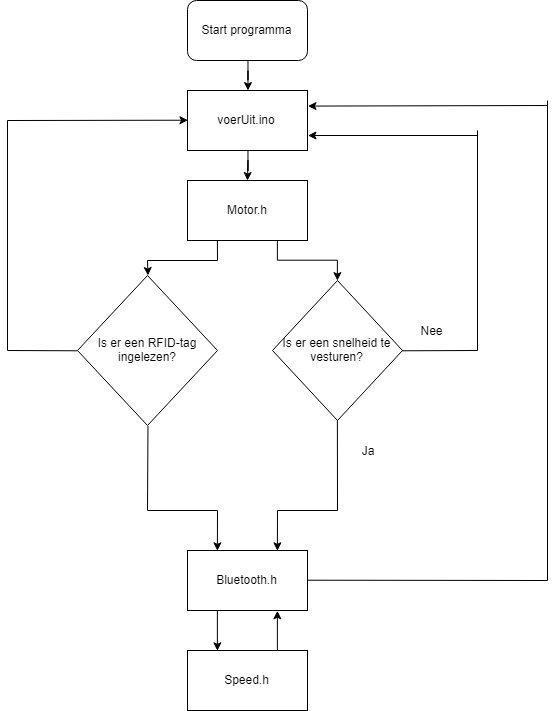
\includegraphics[width=0.5\textwidth]{flowchartLibraries.png}
\caption{Flowchart van de werking van de libraries. \label{fig:flowchart}}
\end{figure}



\subsection{Motor}

We zijn eerst en vooral begonnen met het schrijven van de Motor-bibliotheek. Deze bibliotheek wordt aangeroepen vanuit de loop van het main programma genaamd voerUit.ino. We registreren, elke keer dat de loop wordt uitgevoerd, de digitale waarden aan de sensoren en plaatsen deze voortdurend in de array van integers, genaamd LFS[ ], die vervolgens eenvoudig gebruikt kan worden voor de verwerking en generatie van de effectieve correctiewaarden. Ik stel dergelijke array voor als volgt: 000 001 waarbij nu enkel de meest rechtse infrarood sensor wit detecteert en alle 5 de andere sensoren zwart detecteren. We hebben het programma opgebouwd volgens het principe waarbij we aan de verschillende combinaties van sensoren die wit detecteren, verschillende foutwaarden associ\"eren zodat er in principe geen enkele rusttoestand is. Er wordt als het ware voortdurend gecorrigeerd maar in zo een kleine mate dat dit amper zichtbaar is voor ons. In ons programma krijgt de kleinste fout, namelijk de buitenste sensor die wit detecteert, de foutwaarde 1.1. In het allerslechtste geval, namelijk 000 100, waarbij een van de middelste sensoren wit detecteert, krijgt deze situatie een foutwaarde van 4.6 mee. Deze error values worden elke keer dat het programma doorlopen wordt, aangepast indien de toestand van \'e\'en van de sensoren gewijzigd werd. Deze waarden zijn niet zomaar gekozen maar we hebben uitgezocht welke combinatie van PD-constanten en error values tot de beste prestaties kon leiden. Een voorbeeld van dergelijke code vindt u in Listing \ref{listing:detectiealgoritme}. De error value die gegenereerd werd, wordt vervolgens gebruikt in de corrigeer-methode waarin de werking van ons PD-algoritme in verwerkt zit.

\lstinputlisting[basicstyle=\tiny ]{detectiealgoritme.txt}
\begin{lstlisting}[caption={Het algoritme die de foutwaarden toekent aan de verschillende situaties} \label{listing:detectiealgoritme}]
\end{lstlisting}

\subsection{PD-algoritme}

Dit algoritme is vrij beknopt maar toch zeer interessant aangezien het de prestaties van het wagentje heel erg verbetert. PID is de afkorting voor Proportioneel, Integrerend en Differenti\"erend. Deze regelaar is dus in staat om verschillende soorten fouten te detecteren en in de juiste mate te reageren om zo oscillaties weg te werken en een stabiel voertuig te verkrijgen. Het proportioneel aandeel in de regelaar is een vermenigvuldiging van KP met het verschil van de waarde die je zou willen dat de sensoren meten, verminderd met de waarde die effectief geregistreerd wordt. De integrerende actie zorgt voor een foutcorrectie die ontstaat door het constant optellen van de fout. Hoe langer een fout zich dus voordoet, des te groter de waarde van de integrerende term zal zijn. Ook deze waarde wordt nog vermenigvuldigd met een constante namelijk KI. Als laatste hebben we nog de differenti\"erende term. Deze term is functie van de snelheid van verandering van de fout. Wanneer de afwijking tussen de gewenste waarde en de gemeten waarde toeneemt, zal de D-term in functie van de snelheid van verandering reageren om zo een mogelijks zeer groot wordende fout te beperken in grootte. Ook in de andere richting zal de correctie afgeremd worden wanneer de gemeten waarde nadert naar de gewenste waarde. 

De P-waarde wordt gelijkgesteld aan de error value die we hierboven ge\"introduceerd hebben. De I-waarde hebben we in dit project niet gebruikt aangezien deze waarde enorm snel toeneemt en niet eenvoudig was om perfect in te stellen. Achteraf gezien bleek deze term niet noodzakelijk om een stabiel rijdende robot te verkrijgen. We maken dus gebruik van een PD-regelaar niet van een PID-regelaar. De D-waarde wordt slechts om de 500 milliseconden vervangen door een nieuwe waarde. Mochten we deze tijdsrestrictie niet verwerkt hebben in de code, dan zou de D-waarde amper invloed hebben aangezien ons programma meer dan 1000 keer per seconde wordt uitgevoerd en dus met andere woorden, wanneer de fout gedetecteerd wordt en de D-waarde zijn correctie wilt uitvoeren, er onmiddellijk een nieuwe waarde wordt geregistreerd die meestal opnieuw diezelfde waarde is waardoor de D-correctiewaarde wegvalt. We testten de snelheid van ons programma uit met behulp van onderstaande code om tot dergelijk inzicht te komen en verkregen een uitvoer in de Seri\"ele monitor van 0 milliseconden wat dus illustreert dat het programma meer dan 1000 keer per seconde wordt uitgevoerd.

\lstinputlisting[basicstyle=\tiny ]{tijdsmeting.txt}
\begin{lstlisting}[caption={Het algoritme om de frequentie van de uitvoering van het programma te bepalen} \label{listing:tijdsmeting}]
\end{lstlisting}

De D-waarde en de P-waarde worden vervolgens nog vermenigvuldigd met de KP en KD constanten, zoals te zien in Listing \ref{listing:PID},  die we met behulp van beproeving hebben bepaald om de beste prestaties te verkrijgen. De som van deze producten wordt opgeslagen in PIDvalue en wordt meegegeven in de rij-methode. Wat niets anders is dan een methode voor het instellen van de algemene snelheid en de snelheid per wiel, rekening houdend met de PIDvalue die we net definieerden. 

\lstinputlisting[basicstyle=\tiny ]{PID.txt}
\begin{lstlisting}[caption={Het PD-algoritme dat wij hanteren} \label{listing:PID}]
\end{lstlisting}


\subsection{Detectie-algoritme}

Een extra functionaliteit die we verwerkt hebben in onze code die van belang is bij de error value, is het feit dat als alle sensoren zwart detecteren dat de robot weet of hij zich nu binnen of buiten het parcours bevindt waardoor zijn error values verschillen. Bij alle verschillende situaties waarin de sensoren zich kunnen bevinden, wordt er een boolean aangepast. Zo zal de boolean limitReached in alle gevallen false zijn behalve in de 2 gevallen 000 100 en 001 000, dan zal de boolean true gemaakt worden. Dit zijn de situaties waarbij de robot over de buitenlijn aan het gaan is en de ene arm zich buiten het parcours bevindt en de andere arm zich binnen bevindt. Indien de fout nog een klein beetje verder toeneemt verkrijg je de situatie 000 000 waarbij de witte lijn zich tussen de sensoren bevindt. De robot zal nu zeer hevig gaan corrigeren aangezien de boolean limitReached true is. 

Wanneer we werken met 2 armen ontstaan er extra problemen, namelijk naar welke arm moet er geluisterd worden en in welke richting moet de robot uitwijken wanneer alle sensoren zwart zijn. Elke keer dat er een arm wit registreert, wordt de boolean rechtersensorActief aangepast naar true of false naargelang de arm die het wit detecteert. Wanneer de sensoren volgende situatie registreren 000 001, dan wordt de boolean rechtersensorActief op true gezet. Wanneer je in dit geval los komt van de lijn, weet het programma dat het naar rechts moet gaan corrigeren om de rechterlijn terug te intercepten. Maar wanneer de boolean limitReached op true staat, wilt dat zeggen dat de situatie 000 100 zich net voordien heeft voorgedaan en het wagentje zich dus eigenlijk te ver rechts van het circuit bevindt. Nu zal het wagentje naar links moeten corrigeren met een grotere factor dan normaal aangezien de boolean limitReached deze hevige reactie genereert.


De 2e functionaliteit dat we hebben toegevoegd is het principe dat de robot weet of hij zich links of rechts van de lijn bevindt en zo dus in de juiste richting kan corrigeren. Dit was nodig om de 2 armen te kunnen laten samenwerken.


\subsection {Communicatie}

In de methode bepaalPID() bevinden er zich nog 2 andere methodes die aangeroepen worden, namelijk verstuurSnelheid() en verstuurTag(). Beide methodes bevatten een methode die de communicatie met de Bluetooth-bibliotheek afhandelt. In verstuurSnelheid() bevindt zich de methode bluetooth.stuurSnelheid(). In de Bluetooth-bibliotheek wordt er vervolgens een waarde opgevraagd van de Speed-bibliotheek waarin zich het algoritme voor de registratie van de huidige snelheid van de robot bevindt die je vindt in Listing \ref{listing:snelheidsregistratie}. De snelheidswaarde wordt telkens wanneer het wieltje een rotatie maakt aangepast met behulp van een eenvoudige snelheidsvergelijking. De snelheid wordt vervolgens 1 keer per seconde gereturned naar de Bluetooth-bibliotheek van waar het met behulp van Software Serial verstuurd wordt met de HC-05 naar de Raspberry Pi. 

\lstinputlisting[basicstyle=\tiny ]{snelheidsregistratie.txt}
\begin{lstlisting}[caption={Methode om de snelheid te registreren} \label{listing:snelheidsregistratie}]
\end{lstlisting}

De verstuurTag()-methode is een methode die instaat voor het correct versturen van de RFID-ID van de tags die zich onder de mat bevinden. We stootten daarbij op het probleem dat de mfrc522 gebruikt maakt van de SPI-pinnen. Deze pinnen waren echter reeds in gebruik door de motoraansturing die verwerkt is in onze printplaat en volledig geroute was. De RFID-lezer anders aansluiten was geen optie alsook de printplaat opnieuw routen zagen we niet onmiddellijk zitten. We hebben vervolgens geopteerd om een hulp-arduino te maken die vervolgens zou instaan voor het lezen van de RFID-tags en deze informatie vervolgens via UART, met behulp van de TX-pin, te verzenden naar de RX-pin van de hoofd-Arduino. Hierdoor hebben we het probleem van de SPI-pinnen kunnen oplossen en hebben we via een eenvoudig protocol, communicatie tot stand gebracht tussen beide Arduino's. De ID-waarde die de hoofd-Arduino vervolgens ontvangt, wordt naar de Bluetooth-bibliotheek geleid vanwaar het via Bluetooth verzonden wordt naar de Raspberry Pi.

\lstinputlisting[basicstyle=\tiny ]{communicatie.txt}
\begin{lstlisting}[caption={Algoritme voor het versturen van data via de HC-05 naar de Raspberry Pi} \label{listing:communicatie}]
\end{lstlisting}

\section{Raspberry Pi}


Om de Raspberry Pi werkende te krijgen, hebben we eerst enkele packages moeten installeren om het mogelijk te maken een seri\"ele Bluetooth communicatie tot stand te brengen. Eerst en vooral installeerden we een Bluetooth Interface met behulp van onderstaand commando.

\lstinputlisting[ ]{installbluetooth.txt}
\begin{lstlisting}[ ]
\end{lstlisting}

We kunnen nu via preferences onze bluetooth apparaten beheren en pairen met de HC-05 van onze Arduino. Van zodra we verbonden zijn, komt er een melding dat we gebruik maken van rfcomm0. Deze naam hebben we ook nodig om ons Python programma te laten samenwerken met de Bluetoothchip op de Raspberry Pi. 

Het Python programma is bij ons vrij beknopt. Het is een programma dat voortdurend luistert of er data binnenkomt via Bluetooth en indien er data binnenkomt, deze data vervolgens onmiddellijk afprint. De 2 enige momenten waarbij de Raspberry Pi dus data ontvangt is de snelheid die elke seconde doorgestuurd wordt en elke keer er over een RFID-tag gereden wordt waarbij de ID doorgestuurd wordt. Het Python programma waarvan wij gebruik gemaakt hebben vindt u in Listing \ref{listing:raspberrypicode}

\lstinputlisting[basicstyle=\tiny ]{raspberrypicode.txt}

\begin{lstlisting}[caption={Code die wordt uitgevoerd door de Raspberry Pi} \label{listing:raspberrypicode}]
\end{lstlisting}




%second chapter of your thesis
\chapter{Moeilijkheden}\label{Moeilijkheden}
\section{Software}
Het probleem met de integrator is iets waar we niet dieper op zijn ingegaan en niet hebben opgelost. Het probleem dat zich voordoet is het feit de I-waarde die we genereren, telkens de som is van de fout die zich voordoet. Aangezien de code meer dan 1000 keer per seconde wordt uitgevoerd kan deze waarde in een mum van tijd een extreem grote waarden aannemen wat niet gunstig is voor de robot. Het effect van dit probleem op onze robot was dat hij plots extreem versnelde en onmiddellijk alle controle verloor. We zouden dit probleem kunnen oplossen door de I-waarde voldoende klein te kiezen en eventueel slechts om de zoveel tijd deze waarde aan te passen. Na herhaaldelijke pogingen om dit probleem op te lossen hebben we ingezien dat de I-waarde geen noodzakelijk onderdeel is voor een stabiel rijdende robot en hebben we dus besloten dit weg te laten.

Op het moment dat we onze PD-waarden aan het optimaliseren waren, is er een kortsluiting ontstaan in onze Arduino en motor shield terwijl de batterij was aangesloten. De batterij heeft toen een te grote stroom door beide printplaten gestuurd waardoor deze stuk gingen. Ook 3 sensoren gingen toen stuk. We hebben toen een hele middag gezocht of er een mogelijkheid was om alsnog het motorshield te herstellen aangezien er geen werkende shields op overschot waren. Jammer genoeg was het de L298 die stuk was en hebben we dan een motor shield gekregen waarbij het kroonsteentje stuk was. Na een kleine opknapbeurt hadden we opnieuw een werkende motorshield ter onze beschikking. Onze PD-waarden waren hierdoor weer niet optimaal en hebben dus 2 dagen verloren aan dit gebeuren.

Aangezien we gebruik maken van 2 armen voor het detecteren van beide lijnen van het parcours ontstaat er het probleem dat er 1 arm een hogere prioriteit heeft ten opzichte van de andere arm. De code die we ge\"implementeerd hebben zorgt ervoor dat de rechterarm prioriteit heeft boven de linkerarm aangezien de code voor de rechterarm eerst wordt uitgevoerd. Van zodra er 1 sensor actief is van deze arm, zal de code voor de registratie van de sensoren van de linkerarm zelfs niet meer uitgevoerd worden. Dit heeft er voor gezorgd dat onze robot een voorkeursrichting, namelijk tegenwijzerzin, heeft waarin hij met grotere zekerheid de parcours foutloos zal kunnen afleggen. Wanneer we de buitenbocht volgen, wat meestal het geval is, dan bestaat de kans dat bij een plotse scherpe bocht naar links, de robot onvoldoende corrigeert en daardoor met zowel zijn rechterarm, de buitenlijn detecteert, als met zijn linkerarm, de middellijn detecteert. Deze situatie zou tot geen probleem leiden aangezien zijn rechterarm prioritair is en dus de wit-detectie van zijn linkerarm teniet gedaan wordt. Omgekeerd daarentegen, wanneer links de buitenbocht is bijvoorbeeld 010 100, en hij komt met zijn rechterarm op de middellijn terecht, dan zal de robot de verkeerde kant uitschieten aangezien hij met een grote factor wordt gecorrigeerd omdat de sensor die de extreme situatie voorstelt, oplicht. Gelukkig zijn de sensor-armen instelbaar en konden we per circuit de richting en afstand van de armen instellen om zo optimale prestaties te verkrijgen zonder het probleem van prioriteit uit de kant te ruimen. Een mogelijkheid om dit probleem aan te pakken was om bij te houden met een boolean welke arm er actief is en welke arm er net nieuw contact maakt met de witte lijn. De arm die bijvoorbeeld al het langst actief was, kunnen we dan als prioritaire arm beschouwen en elke keer dat we de situatie 000 000 tegenkomen, wat overeenkomt met alle sensoren die zich in het zwart bevinden, kan de prioriteit van de arm opnieuw ingesteld worden.

Voor het eenvoudigste, ovale circuit hadden we onze code geoptimaliseerd op 72. Deze snelheid komt overeen met 0.48 m/s en was een zeer hoge snelheid als je onze robot zag rondrijden. Wanneer we vervolgens het 2e circuit te zien kregen werd het duidelijk dat de robot dit circuit niet aan deze snelheid zou kunnen afleggen. We verlaagden onze snelheid dan naar 65, zodat de robot zonder fouten dit 2e circuit zou kunnen afleggen. Deze snelheidsvermindering ging ook gepaard met nieuwe PD-waarden en we konden met andere woorden opnieuw beginnen met het instellen van de robot. Het probleem waar we nu mee te maken kregen, is dat we een lager vermogen hadden voor de motoren en dus bij sommige grote bulten een duwtje moesten geven om onze robot zijn rit te laten verderzetten. De snelheid opdrijven, zou resulteren in het opnieuw aanpassen van de error values en PD-waarden, waardoor we besloten genoegen te nemen met een snelheid van 0.28 m/s.

Op het moment dat onze printplaat, Arduino gecombineerd met een motor shield, klaar was, wilden we de RFID-lezer connecteren met de Arduino. We stuitten op het probleem dat de RFID-lezer gebruik maakt van de pinnen: 9, 10, 11,12 en 13 terwijl we onze printplaat reeds geroute hadden waarbij de pinnen 11 12 en 13 intern verbonden waren met de L298. Dit vormde een groot probleem aangezien het voor de RFID-lezer niet mogelijk was gebruik te maken van andere pinnen aangezien die gebruikt maakt van SPI. Dit probleem konden we oplossen door onze routing volledig opnieuw te doen waarbij we andere pinnen zouden gebruiken om de L298 aan te sturen. Aangezien daar geen tijd voor was, bedachten we dat we konden gebruik maken van een andere hulp-Arduino die instond voor het lezen van de RFID-tags en voor het verzenden via UART naar de hoofd-Arduino. Deze hoofd-Arduino verloor met als gevolg dus slechts 1 pin, namelijk de RX-pin, aan het lezen van de RFID-tags. Aangezien we voordien reeds een prototype-Arduino gemaakt hadden, konden we deze gebruiken als hulp-Arduino en konden we op het einde van de rit alsnog ons project afronden waarbij we enkel gebruik maakten van zelfgemaakte printplaten.

Wanneer we data via Bluetooth verzonden van de Raspberry Pi naar de Arduino en omgekeerd stootten we op het probleem dat er regelmatig karakters fout waren ontvangen en de communicatie dus niet optimaal was. We hebben vervolgens trachten te achterhalen wat het probleem exact was. We merkten op dat de RX- en TX-pinnen, waaraan wij de Bluetooth module hadden aangesloten, ook rechtstreeks verbonden zijn met de USB-poort. Wanneer we dus met behulp van Serial.println(), data wilden wegschrijven naar de seri"ele monitor, gebeurde dat als het ware op dezelfde datalijn als de data die we ontvingen via de Bluetooth module. We konden dit probleem oplossen door niet langer gebruik te maken van Hardware Serial maar wel door Software Serial waarbij we de pinnen A2 en 2 gebruikten als respectievelijk RX en TX.

\section{Hardware}
We waren er ons van bewust dat het vrijwel onmogelijk was dat onze PCB geen kinderziekten zou vertonen bij ons eerste ontwerp. De problemen kwamen vrijwel onmiddellijk tot uiting bij de L298. Het ground-vlak viel wat groter uit dan door de footprint voorzien was waardoor dit vlak contact maakte met een baan waarover +5V stond en dus eigenlijk kortsluiting vormde. We hebben dit probleem kunnen oplossen door plakband tussen het ground-vlak en het baantje te kleven om zo het contact te verbreken. Hoewel de oplossing niet ideaal was, waren we hiermee wel geholpen. We hebben dan onmiddellijk de footprint gewijzigd zodat onze finale PCB dit probleem niet zou vertonen. We hadden ook problemen met de reset-knop waarbij de afmetingen van de gebruikte footprint niet klopten. We hebben dit opgelost door gebruik te maken van een drukknop met slechts twee pinnen die verbonden worden met elkaar bij het indrukken van de knop. 

Bij het testen van de PCB merkten we vrijwel onmiddellijk op dat een paar componenten warm werden. Dit was een directe indicatie van het feit dat de printplaat nog niet op punt stond. We hebben na lang zoeken en met hulp van onze coach, 3 problemen ontdekt. We hebben deze problemen ook aangeduid op figuur??%~\ref{fig:PCBProblemen}
Probleem 1 was een Schottky-diode die niet goed verbonden was met zijn baantje. De diode maakte soms wel contact en soms niet. Daar de footprint van de diode nog steeds te klein uitviel hebben we het probleem opgelost door een draadje te solderen aan de contactzijde om zo veen verbinding te maken met de baan.
Probleem 2 was simpelweg een Via die we over het hoofd gezien hadden waardoor een pin van de L298 niet verbonden was. 
Probleem 3 was het de grootste boosdoener. We waren in het schema \'e\'en label vergeten te plaatsen waardoor de L298, die in staat voor de motorsturing, niet gevoed werd met PWRIN. Hierdoor werden de signalen niet goed verwerkt door de L298 en kregen de motoren dus ook niet de juiste signalen. We hebben dit nogmaals opgelost door een verbinding te solderen tussen de IC en de PWRIN. De PWRIN is het signaal dat rechtstreeks via de kroonsteentjes binnenkomt van de batterij.





%second chapter of your thesis
\chapter{Coach}
In het vorig hoofdstuk hebben we naar deze tekst verwezen\label{verwijzing}.

%second chapter of your thesis
\chapter{Besluit}
We kunnen terugkijken op een zeer leerrijke en toch wel zeer plezante bachelorproef. De twee aspecten van Elektronica zaten erin verwerkt, nl. hardware maar ook een belangrijk deel software. We hebben ook enkele testjes uit moeten voeren om bijvoorbeeld te beslissen hoe we de sensors moesten plaatsen, ver/dicht van het wagentje, schuin of recht,\ldots Dan moesten we ook zelf beslissen welke modules we gebruikten, wat we wel en wat niet zelf moesten maken. We hebben toch wel de meeste foutjes en problemen tegengekomen die iedereen in een leerproces moet meemaken. Bij ieder nieuw PCB-design zitten er wel altijd enkele foutjes, dit was in ons geval natuurlijk niet anders. Sommige problemen konden we zeer snel en gemakkelijk oplossen, andere problemen hebben bloed, zweet en tranen gekost om te vinden en op te lossen. Bij het software onderdeel was het vooral de uitdaging om de PID (in ons geval PD) afregeling te doen, vooral omdat we dit nog in geen enkel vak in theorie hadden gezien. We kunnen wel met een positieve blik terugkijken op onze vormgeving en afregeling van ons wagentje. We waren over alle vier de parcours die we voorgeschoteld kregen de snelste, we moeten er wel bij vertellen dat we 4x uit het parcours zijn geraakt. Twee keer meer dan de tweede groep die in het totaal 2x uit het parcours ontsnapte. Kortom uit deze bachelorproef hebben we volgende zaken geleerd: PID afregelen, Bluetooth connectie maken met RPI, RFID-tags uitlezen, PCB ontwerpen, PCB debuggen, SMD solderen, 3D-printen. 
 


% Bibliografie: referenties. De items zitten in bibliografie.bib
%%%%%%%%%%%%%%%%%%%%%%%%%%%%%%%%%%%%%%%%%%%%%%%%%%%%%%%%%%%%%%%%%
% Indien je ook de niet geciteerde werken in je bibliografie wil opnemen, commentarieer dan onderstaande regel uit!
%\nocite{*}
%\bibliographystyle{apalike}
%\bibliography{bibliografie}

% Eventueel enkele appendices
%%%%%%%%%%%%%%%%%%%%%%%%%%%%%%
\appendix
%\input{bijlage1}

% Bijlage met daarin het wetenschappelijk artikel
%%%%%%%%%%%%%%%%%%%%%%%%%%%%%%%%%%%%%%%%%%%%%%%%%%
%\chapter{Beschrijving van deze masterproef in de vorm van een wetenschappelijk artikel}
%\includepdf{artikel.pdf}

% Bijlage met daarin de poster
%%%%%%%%%%%%%%%%%%%%%%%%%%%%%%%
%\chapter{Poster}
%\includepdf{poster.pdf}


\includepdf{back_fiiw_gent.pdf}
% \includepdf{back_fiiw_ghent_eng.pdf} % For the english version

\end{document}
